\section{The group $\Gamma_1(6)$}

This group is exactly the subgroup of $\SL_2(\bZ)$ of all matrices $(\begin{smallmatrix}
    a & b \\ c & d
\end{smallmatrix})$ with $a \equiv d \equiv 1 \pmod{6}$, $c \equiv 0 \pmod{6}$.
Its fundamental domain can be pictured as below.

% Inspired from https://tex.stackexchange.com/a/661303/111403
\begin{center}
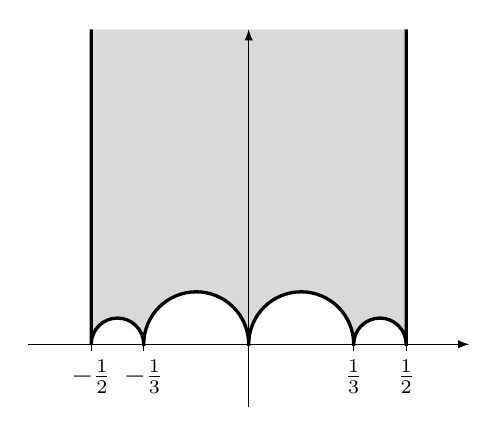
\begin{tikzpicture}[scale=4]
    \draw[very thick, fill=gray!30]
        (-.5,1) -- (-.5,0) --
        (-1/2, 0) arc (180:0:1/12) --
        (-1/3, 0) arc (180:0:1/6) --
        (0, 0) arc (180:0:1/6) --
        (1/3, 0) arc (180:0:1/12) --
        (.5, 0) -- (.5,1);
    \draw[-latex] (-0.7,0) -- (0.7,0);
    \draw[-latex] (0,-.2) -- (0,1);
    \draw(-.5,.02)--(-.5,-.02)node[below]{$-\frac{1}{2}$};
    \draw(.5,.02)--(.5,-.02)node[below]{$\frac{1}{2}$};
    \draw(-1/3,.02)--(-1/3,-.02)node[below]{$-\frac{1}{3}$};
    \draw(1/3,.02)--(1/3,-.02)node[below]{$\frac{1}{3}$};
\end{tikzpicture}
\end{center}
A complete set of inequivalent cusps is given by $0, 1/2, 1/3, \infty$.
They are regular and have widths 6, 3, 2, 1 respectively.
Consider the following function
$$
    y(\tau) = \frac{\eta(6\tau)^8 \eta(\tau)^4}{\eta(2\tau)^6 \eta(3\tau)^4}
$$
where
$$
    \eta(\tau) = q^{1/24} \prod_{n=1}^{\infty} (1 - q^n), \quad q = e^{2\pi i \tau}, \quad \tau \in \bH.
$$
That it is a modular function on $\Gamma_1(6)$ can be checked using the tranformation formula for $\eta(\tau)$ in \cite[Ch 9]{rademacher2012topics}.
Since $y(\tau)$ has only one simple zero in the fundamental domain it generates the field of modular functions on $\Gamma_1(6)$.
Moreover, $y(0) = \frac{1}{9}$, $y(\frac{1}{3}) = 1$, $y(\frac{1}{2}) = \infty$, $y(\infty) = 0$.
The function $y(-\frac{1}{6\tau})$ is again invariant on $\Gamma_1(6)$ and one easily checks that
\begin{equation}
    \label{eqn:1}
    y\left(-\frac{1}{6\tau}\right) = \frac{y(\tau) - 1/9}{y(\tau) - 1}.
\end{equation}
Hence the function
$$
    t(\tau) = y(\tau) \frac{1 - 9y(\tau)}{1 - y(\tau)}
$$
is invariant under the involution $\tau \mapsto -1/6\tau$.
Moreover,
$$
    t(\tau) = \left(\frac{\Delta(6\tau) \Delta(\tau)}{\Delta(3\tau) \Delta(2\tau)}\right)^{1/2} = q \prod_{n = 0}^{\infty} (1 - q^{6n + 1})^{12} (1 - q^{6n + 5})^{-12}
$$
which is checked by noticing that $(\Delta(6\tau) \Delta(\tau) / \Delta(3\tau) \Delta(2\tau))^{1/2}$ is modular with respect to $\Gamma_1(6)$, invariant under $\tau \mapsto -1/6\tau$ and its zeros and poles coincide with those of $t(\tau)$.

\begin{proposition}
\label{prop:2.1}
    The function $t(\tau)$ maps the shaded open area in the picture below univalently onto the upper half plane and satisfies
    $$
        t(i\infty) = 0, \quad t\left(\frac{i}{\sqrt{6}}\right) = (\sqrt{2} - 1)^{4}, \quad t\left(\frac{2}{5} + \frac{i}{5\sqrt{6}}\right) = (\sqrt{2} + 1)^{4},\quad t\left(\frac{1}{2}\right) = \infty.
    $$
\end{proposition}
\begin{center}
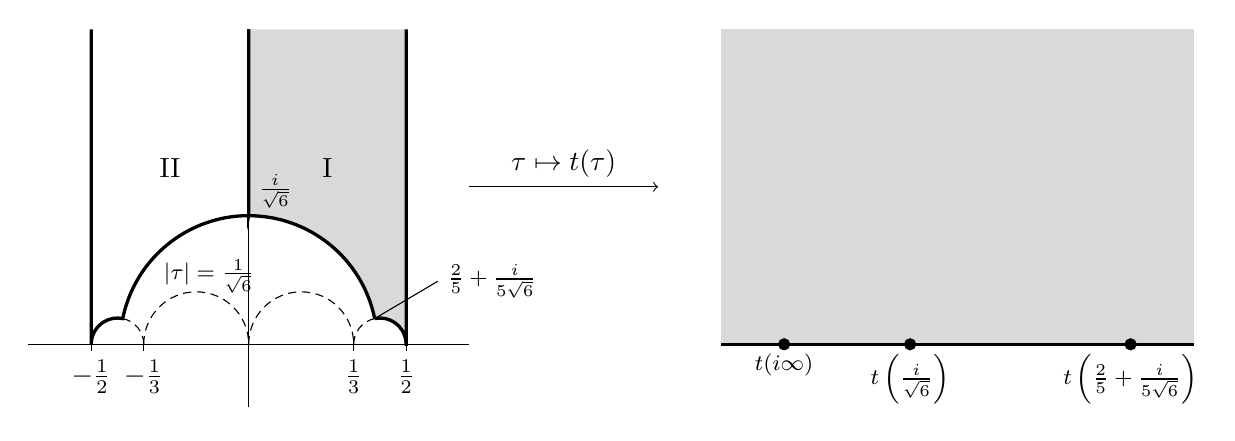
\begin{tikzpicture}[scale=4]
    \draw[very thick]
        (-.5,1) -- (-.5,0) --
        (-1/2, 0) arc (180:78.5:1/12) --
        (-2/5, {1/(5 * sqrt(6))}) arc (168.5:90:{1/sqrt(6)}) --
        (0,{1/sqrt(6)}) -- (0,1);
    \draw[very thick, fill=gray!30]
        (0,1) --
        (0, {1/sqrt(6)}) arc (90:11.5:{1/sqrt(6)}) --
        (2/5, {1/(5 * sqrt(6))}) arc (101.5:0:1/12) --
        (1/2,0) -- (1/2,1);
    \draw (-0.7,0) -- (0.7,0);
    \draw (0,-.2) -- (0,1);
    \draw (0,0.4)node[above right, font=\footnotesize]{$\frac{i}{\sqrt{6}}$};
    \draw[densely dashed] (-1/3, 0) arc (0:78.5:1/12);
    \draw[densely dashed] (-1/3,0) arc (180:0:1/6);
    \draw[densely dashed] (1/3,0) arc (180:101.5:1/12);
    \draw[densely dashed] (0,0) arc (180:0:1/6);
    \draw(-.5,.02)--(-.5,-.02)node[below]{$-\frac{1}{2}$};
    \draw(.5,.02)--(.5,-.02)node[below]{$\frac{1}{2}$};
    \draw(-1/3,.02)--(-1/3,-.02)node[below]{$-\frac{1}{3}$};
    \draw(1/3,.02)--(1/3,-.02)node[below]{$\frac{1}{3}$};
    \draw (2/5, {1/(5 * sqrt(6))}) -- (0.6,0.2)node[right, font=\footnotesize]{$\frac{2}{5} + \frac{i}{5\sqrt{6}}$};
    \draw (-0.25, 0.5)node[above]{II};
    \draw (0.25, 0.5)node[above]{I};
    \draw (-0.3, 0.3)node[below right, font=\footnotesize]{$|\tau| = \frac{1}{\sqrt{6}}$};

    \draw[->] (0.7,0.5) -- (1.3,0.5);
    \draw (1.0, 0.5)node[above]{$\tau \mapsto t(\tau)$};

    \fill[gray!30] (1.5,1.0) -- (1.5,0) -- (3.0, 0) -- (3.0, 1.0);
    \draw[very thick] (1.5,0) -- (3,0);
    \draw[fill] (1.7,0) circle (0.5pt)node[below, font=\footnotesize]{$t(i\infty)$};
    \draw[fill] (2.1,0) circle (0.5pt)node[below, font=\footnotesize]{$t\left(\frac{i}{\sqrt{6}}\right)$};
    \draw[fill] (2.8,0) circle (0.5pt)node[below, font=\footnotesize]{$t\left(\frac{2}{5}+\frac{i}{5\sqrt{6}}\right)$};
\end{tikzpicture}
\end{center}

\begin{proof}
That $t(i \infty) = 0$, $t(\frac{1}{2}) = \infty$ can be ssen from the values $y(i\infty) = 0$, $y(\frac{1}{2}) = \infty$.
From \eqref{eqn:1} it follows that for $\tau = \frac{i}{\sqrt{6}}$ and $y_0 = y(\frac{i}{\sqrt{6}})$, we have $y_0 = \frac{y_0 - \frac{1}{9}}{y_0 - 1}$, hence $y_0 = 1 \pm \frac{2 \sqrt{2}}{3}$ and correspondingly, $t(\frac{i}{\sqrt{6}}) = (\sqrt{2} \pm 1)^4$.
The same principle can be applied to obatin $t(\frac{2}{5} + \frac{i}{5\sqrt{6}}) = (\sqrt{2} \pm 1)^4$.
To decide which sign should be taken, one estimates $t(\frac{i}{\sqrt{6}})$ and $t(\frac{2}{5} + \frac{i}{5\sqrt{6}})$ numerically and obtain the values of our proposition.
Furthermore, $t(\tau)$ assumes every value at most once in the union of I and II.
Our proposition now follows.
\end{proof}

In the theorems and proofs that follow we let $\rM_k(\Gamma_1(6))$ be the space of modular forms of weight $k$ with respect to $\Gamma_1(6)$, and let
$$
    E_4 (\tau) = 1 + 240 \sum_{n=1}^{\infty} \sigma_3(n) q^n, \quad E_2(\tau) = 1 - 24 \sum_{n=1}^{\infty} \sigma_1(n) q^n 
$$
be the standard Eisenstein series.

\begin{theorem}
    \label{thm:1}
    $\zeta(3)$ is irrational.
\end{theorem}

\begin{proof}
    Let
    \begin{align*}
        40 F(\tau) &= E_4(\tau) - 36 E_4(\tau) - 7 (4E_4(2\tau) - 9E_4(3\tau)) \\
        24 E(\tau) &= -5(E_2(\tau) - 6E_2(6\tau)) + 2E_2(2\tau) - 3E_2(3\tau).
    \end{align*}
    Notice that $F(\tau) \in \rM_4(\Gamma_1(6))$ and $F(-\frac{1}{6\tau}) = -36 \tau^4 F(\tau)$, $F(i\infty) = 0$ and $E(\tau) \in \rM_2(\Gamma_1(6))$, $E(-\frac{1}{6\tau}) =  - 6\tau^2 E(\tau)$.
    The Dirichlet series corresponding to $F(\tau)$ reads
    \begin{align*}
        L(F, s) &= \sum_{n=1}^{\infty} \frac{6\sigma_3(n)}{n^s} - 36 \frac{6 \sigma_3(n)}{(6n)^s} - 28 \frac{6 \sigma_3(n)}{(2n)^s} + 63 \frac{6 \sigma_3(n)}{(3n)^s} \\
        &= 6(1 - 6^{2-s} - 7 \cdot 2^{2-s} + 7 \cdot 3^{2-s}) \zeta(s) \zeta(s - 3).
    \end{align*}
    Define $f(\tau)$ by $(\frac{\dd}{\dd \tau})^{3} f(\tau) = (2 \pi i )^{3} F(\tau)$, $f(i \infty) = 0$.
    From Proposition \ref{prop:1.2} and the fact that $F(-\frac{1}{6\tau}) = -36 \tau^4 F(\tau)$ follows\footnote{There's a typo in the original article: $L(F, s)$ should be $L(F, 3)$.}
    $$
        6 \tau^2 \left(f\left(-\frac{1}{6\tau}\right) - L(F, 3)\right) = -(f(\tau) - L(F, 3))
    $$
    and since $L(F, 3) = 6 \cdot (-1/3) \zeta(3) \zeta(0) = \zeta(3)$, we have
    $$
        6 \tau^2 \left(f\left(-\frac{1}{6\tau}\right) - \zeta(3)\right) = -(f(\tau) - \zeta(3)).
    $$
    Multiplication with $E(-1/6\tau) = -6\tau^2 E(\tau)$ gives
    \begin{equation}
        \label{eqn:2}
        E\left(-\frac{1}{6\tau}\right) \left(f\left(-\frac{1}{6 \tau}\right) - \zeta(3)\right) = E(\tau) (f(\tau) - \zeta(3)).
    \end{equation}
    The function $E(\tau)(f(\tau) - \zeta(3))$ can be considered as a multivalued function of $t = t(\tau)$.
    We choose it at $t = 0$ as follows.
    From the expansion $t = q\prod_{n=1}^{\infty} (1 - q^{6n + 1})^{12} (1 - q^{6n + 5})^{-12} = q - 12q^2 + 66q^3 - 220q^4 + 495 q^5 - \dots$ one infers the inverse expansion $q = t + 12 t^2 + 222 t^3 + \dots$.
    Then, from $E(\tau) = 1 + 5q + 13 q^2 + \dots$ one finds $E(t) = 1 + 5t + 73 t^2 + 1445 t^3 + \dots$ and similarly, $E(t) F(t) = 6t + (351/4)t^2 + \dots$.

    By construction one notes that $E(t) \in \bZ\llbracket t\rrbracket$ and  and $E(t) f(t) = \sum_{n=1}^{\infty} a_n t^n$ where $a_n \in \bZ / [1, \dots, n]^3$.
    Since the inverse function $t \to \tau$ branches at $(\sqrt{2} - 1)^{4}$ one expects the radius of convergence of $E(t)(f(t) - \zeta(3))$ to be $(\sqrt{2} - 1)^{4}$.
    However, by the property \eqref{eqn:2}, the function $t \mapsto E(t) (f(t) - \zeta(3))$ has no branch point at $t = (\sqrt{2} - 1)^4$, and its radius of convergence equals at least the next branching value, which is $(\sqrt{2} + 1)^{4}$.
    Furthermore, it cannot be a polynomial in $t$, since then $f(\tau) - \zeta(3)$ would be a modular form of weight $-2$, which is impossible.
    We now apply Proposition \ref{prop:1.1} with $\theta_1 = \zeta(3)$ to conclude $\zeta(3) \not \in \bQ$.
\end{proof}

\begin{remark*}
    Note that $1, 5, 73, 1445, \dots$ are exactly Ap\'ery's numbers for $\zeta(3)$.
\end{remark*}

\begin{theorem}
    \label{thm:2}
    Let $F(\tau)  = \eta(\tau)^{2} \eta(2\tau)^{2} \eta(3\tau)^{2} \eta(6\tau)^2$ and $L(F, s)$ the corresponding Dirichlet series.
    Then at least one of the numbers $\pi^{-2}L(F, 2)$ and $L(F, 3) + \frac{47 L(F, 2) \zeta(3)}{48 \pi^2}$ is irrational.
\end{theorem}

\begin{proof}
    The function $F(\tau)$ is in $\rM_4(\Gamma_1(6))$, it is a cusp form, and $F(-\frac{1}{6\tau}) = 36 \tau^4 F(\tau)$.
    Let $f(\tau)$ be the Fourier series such that $(\frac{\dd}{\dd \tau})^{3} f(\tau) = (2 \pi i )^{3} F(\tau)$, $f(i \infty) = 0$.
    Then it follows from Proposition \ref{prop:1.2} that
    \begin{equation}
        \label{eqn:3}
        6 \tau^2 \left(f\left(-\frac{1}{6\tau}\right) - L(F, 3)\right) = f(\tau) - L(F, 3) - L(F, 2) (2 \pi i \tau).
    \end{equation}
    Consider also
    $$
        240 G(\tau) = 13 (E_4(\tau) + 36 E_4(6\tau)) - 37 (4E_4(2\tau) + 9E_4(3\tau)).
    $$
    It ahs the properties $G(i\infty) = 0$, $G(-\frac{1}{6\tau}) = 36 \tau^4 G(\tau)$.
    The corresponding Dirichlet series reads
    $$
        L(G, s) = (13 + 13 \cdot 6^{2-s} - 37 \cdot 2^{2-s} - 37 \cdot 3^{2-s}) \zeta(s) \zeta(s - 3).
    $$
    Letting $(\frac{\dd}{\dd \tau})^{3} g(\tau) = (2\pi i)^{3} G(\tau)$, $g(i\infty) = 0$, we have
    $$
        6 \tau^2 \left(g\left(-\frac{1}{6\tau}\right) - L(G, 3)\right) = g(\tau) - L(G, 3) - L(G, 2) (2 \pi i \tau),
    $$
    hence,
    \begin{equation}
        \label{eqn:4}
        6 \tau^2 \left(g\left(-\frac{1}{6\tau}\right) - \frac{47}{3}\zeta(3)\right) = g(\tau) - \frac{47}{6} \zeta(3) + 48 \zeta(2) (2\pi i \tau).
    \end{equation}
    Elimination of $2\pi i \tau$ form \eqref{eqn:3} and \eqref{eqn:4} gives that the function $h(\tau) = 48 \zeta(2) (f(\tau) - L(F, 3)) + L(F, 2) (g(\tau) - \frac{47}{6}\zeta(3))$ behaves like $6 \tau^2 h(-\frac{1}{6\tau}) = h(\tau)$.
    Now consider
    $$
        E(\tau) = E_2(\tau) - 2E_2(2 \tau) + 6 E_2(3\tau) - 3 E_2(6\tau).
    $$
    It is in $\rM_2(\Gamma_1(6))$ and we have $E(-\frac{1}{6\tau}) = 6 \tau^2 E(\tau)$.
    Consequently, $E(-\frac{1}{6\tau}) h(-\frac{1}{6\tau}) = E(\tau) h(\tau)$ and by an argument to the one in Theorem \ref{thm:1} we find that
    $$
        48 \zeta(2) f(t) E(t) + L(F, 2) g(t) E(t) - \left(48 \zeta(2) L(F, 3) + L(F, 2) \frac{47}{6} \zeta(3) \right) E(t)
    $$
    is a power series in $t$ with radius of convergence $(\sqrt{2} + 1)^4$.
    Again the denominator of the $n$-th coefficient in the power series of $E(t) f(t)$, $E(t) g(t)$, $E(t)$ divides $[1, \dots, n]^3$.
    We can now apply Proposition \ref{prop:1.1} to obtain our theorem.
\end{proof}

\begin{theorem}
    \label{thm:3}
    Let
    $$
        \sum_{n=1}^{\infty} a_n q^n = \left(\frac{\eta^9(\tau) \eta^9 (6\tau)}{\eta^3(2\tau) \eta^3(3 \tau)}\right)^{\frac{1}{2}} = q \prod_{n=1}^{\infty} (1 - q^n)^{3} (1 - q^{3n})^{3} \frac{(1 + q^{3n})^{\frac{9}{2}}}{(1 + q^{n})^{\frac{3}{2}}}.
    $$
    Then $\sum_{n=1}^{\infty} a_n / n^{2}$ is irrational.
\end{theorem}

\begin{proof}
    Consider the product
    $$
        E(\tau) = \frac{\eta^7(2\tau) \eta^7(3 \tau)}{\eta^5(\tau) \eta^5(6\tau)}.
    $$
    We have $E(-\frac{1}{6\tau}) = -6 \tau^2 E(\tau)$ and hence $\sqrt{E(-\frac{1}{6\tau})} = \pm (i \tau \sqrt{6}) \sqrt{E(\tau)}$.
    Since $E(\tau)$ has only zeros and poles in the cusps, it can be well-defined on the upper half plane.
    Since $E(\frac{i}{\sqrt{6}}) \ne 0$, we should have $\sqrt{E(-\frac{1}{6\tau})} = -i \tau \sqrt{6} E(\tau)$. Now consider
    $$
        F(\tau) = \frac{\eta^7(\tau) \eta^7(6\tau)}{\eta^5(2\tau) \eta^5(3\tau)} \sqrt{E(\tau)}
    $$
    which obeys $F(-\frac{1}{6\tau}) = (-i\tau \sqrt{6})^{3} F(\tau)$.
    Let $f(\tau)$ be defined by $(\frac{\dd}{\dd \tau})^{2} f(\tau) = (2 \pi i)^2 F(\tau)$, $f(i\infty) = 0$.
    Then
    $$
        -i\tau \sqrt{6} \left(f\left(-\frac{1}{6\tau}\right) - L(F, 2)\right) = f(\tau) - L(F, 2).
    $$
    Multiplication with $\sqrt{E(-\frac{1}{6\tau})} = -i\tau \sqrt{6} \sqrt{E(\tau)}$ yields\footnote{There's a typo in the original article: $f(\tau)$ on the LHS should be $f(-\frac{1}{6\tau})$.}
    $$
        \sqrt{E\left(-\frac{1}{6 \tau}\right)} \left(f\left(-\frac{1}{6\tau}\right) - L(F, 2)\right) = \sqrt{E(\tau)} (f(\tau) - L(F, 2)).
    $$
    Notice that $\sqrt{E(\tau)}$ considered as a function of $t$ is a power series whose $n$-th coefficient is rational and has denominator dividing $4^n [1, \dots, n]^2$.
    By the same argument as in the previous theorems, the radius of convergence of $\sqrt{E(t)} (f(t) - L(F, 2))$ is at least $(\sqrt{2} + 1)^4$.
    Since $4 e < (\sqrt{2} + 1)^{4}$, we can apply Proposition \ref{prop:1.1} to find our theorem.
\end{proof}

\begin{remark*}
    Theorem \ref{thm:3} is the one alluded to in \cite{beukers1982irrationality}.
\end{remark*}
